%% bare_conf.tex
%% V1.4b
%% 2015/08/26
%% by Michael Shell
%% See:
%% http://www.michaelshell.org/
%% for current contact information.
%%
%% This is a skeleton file demonstrating the use of IEEEtran.cls
%% (requires IEEEtran.cls version 1.8b or later) with an IEEE
%% conference paper.
%%
%% Support sites:
%% http://www.michaelshell.org/tex/ieeetran/
%% http://www.ctan.org/pkg/ieeetran
%% and
%% http://www.ieee.org/

%%*************************************************************************
%% Legal Notice:
%% This code is offered as-is without any warranty either expressed or
%% implied; without even the implied warranty of MERCHANTABILITY or
%% FITNESS FOR A PARTICULAR PURPOSE! 
%% User assumes all risk.
%% In no event shall the IEEE or any contributor to this code be liable for
%% any damages or losses, including, but not limited to, incidental,
%% consequential, or any other damages, resulting from the use or misuse
%% of any information contained here.
%%
%% All comments are the opinions of their respective authors and are not
%% necessarily endorsed by the IEEE.
%%
%% This work is distributed under the LaTeX Project Public License (LPPL)
%% ( http://www.latex-project.org/ ) version 1.3, and may be freely used,
%% distributed and modified. A copy of the LPPL, version 1.3, is included
%% in the base LaTeX documentation of all distributions of LaTeX released
%% 2003/12/01 or later.
%% Retain all contribution notices and credits.
%% ** Modified files should be clearly indicated as such, including  **
%% ** renaming them and changing author support contact information. **
%%*************************************************************************


% *** Authors should verify (and, if needed, correct) their LaTeX system  ***
% *** with the testflow diagnostic prior to trusting their LaTeX platform ***
% *** with production work. The IEEE's font choices and paper sizes can   ***
% *** trigger bugs that do not appear when using other class files.       ***                          ***
% The testflow support page is at:
% http://www.michaelshell.org/tex/testflow/



\documentclass[conference]{IEEEtran}
% Some Computer Society conferences also require the compsoc mode option,
% but others use the standard conference format.
%
% If IEEEtran.cls has not been installed into the LaTeX system files,
% manually specify the path to it like:
% \documentclass[conference]{../sty/IEEEtran}





% Some very useful LaTeX packages include:
% (uncomment the ones you want to load)


% *** MISC UTILITY PACKAGES ***
%
%\usepackage{ifpdf}
% Heiko Oberdiek's ifpdf.sty is very useful if you need conditional
% compilation based on whether the output is pdf or dvi.
% usage:
% \ifpdf
%   % pdf code
% \else
%   % dvi code
% \fi
% The latest version of ifpdf.sty can be obtained from:
% http://www.ctan.org/pkg/ifpdf
% Also, note that IEEEtran.cls V1.7 and later provides a builtin
% \ifCLASSINFOpdf conditional that works the same way.
% When switching from latex to pdflatex and vice-versa, the compiler may
% have to be run twice to clear warning/error messages.



\usepackage[dvipsnames]{xcolor}


% *** CITATION PACKAGES ***
%
\usepackage{cite}
% cite.sty was written by Donald Arseneau
% V1.6 and later of IEEEtran pre-defines the format of the cite.sty package
% \cite{} output to follow that of the IEEE. Loading the cite package will
% result in citation numbers being automatically sorted and properly
% "compressed/ranged". e.g., [1], [9], [2], [7], [5], [6] without using
% cite.sty will become [1], [2], [5]--[7], [9] using cite.sty. cite.sty's
% \cite will automatically add leading space, if needed. Use cite.sty's
% noadjust option (cite.sty V3.8 and later) if you want to turn this off
% such as if a citation ever needs to be enclosed in parenthesis.
% cite.sty is already installed on most LaTeX systems. Be sure and use
% version 5.0 (2009-03-20) and later if using hyperref.sty.
% The latest version can be obtained at:
% http://www.ctan.org/pkg/cite
% The documentation is contained in the cite.sty file itself.






% *** GRAPHICS RELATED PACKAGES ***
%
\ifCLASSINFOpdf
   \usepackage[pdftex]{graphicx}
  % declare the path(s) where your graphic files are
  % \graphicspath{{../pdf/}{../jpeg/}}
  % and their extensions so you won't have to specify these with
  % every instance of \includegraphics
  % \DeclareGraphicsExtensions{.pdf,.jpeg,.png}
\else
  % or other class option (dvipsone, dvipdf, if not using dvips). graphicx
  % will default to the driver specified in the system graphics.cfg if no
  % driver is specified.
  % \usepackage[dvips]{graphicx}
  % declare the path(s) where your graphic files are
  % \graphicspath{{../eps/}}
  % and their extensions so you won't have to specify these with
  % every instance of \includegraphics
  % \DeclareGraphicsExtensions{.eps}
\fi
% graphicx was written by David Carlisle and Sebastian Rahtz. It is
% required if you want graphics, photos, etc. graphicx.sty is already
% installed on most LaTeX systems. The latest version and documentation
% can be obtained at: 
% http://www.ctan.org/pkg/graphicx
% Another good source of documentation is "Using Imported Graphics in
% LaTeX2e" by Keith Reckdahl which can be found at:
% http://www.ctan.org/pkg/epslatex
%
% latex, and pdflatex in dvi mode, support graphics in encapsulated
% postscript (.eps) format. pdflatex in pdf mode supports graphics
% in .pdf, .jpeg, .png and .mps (metapost) formats. Users should ensure
% that all non-photo figures use a vector format (.eps, .pdf, .mps) and
% not a bitmapped formats (.jpeg, .png). The IEEE frowns on bitmapped formats
% which can result in "jaggedy"/blurry rendering of lines and letters as
% well as large increases in file sizes.
%
% You can find documentation about the pdfTeX application at:
% http://www.tug.org/applications/pdftex





% *** MATH PACKAGES ***
%
\usepackage{amsmath}
% A popular package from the American Mathematical Society that provides
% many useful and powerful commands for dealing with mathematics.
%
% Note that the amsmath package sets \interdisplaylinepenalty to 10000
% thus preventing page breaks from occurring within multiline equations. Use:
%\interdisplaylinepenalty=2500
% after loading amsmath to restore such page breaks as IEEEtran.cls normally
% does. amsmath.sty is already installed on most LaTeX systems. The latest
% version and documentation can be obtained at:
% http://www.ctan.org/pkg/amsmath





% *** SPECIALIZED LIST PACKAGES ***
%
\usepackage{algorithmic}
\usepackage{amsmath}
% algorithmic.sty was written by Peter Williams and Rogerio Brito.
% This package provides an algorithmic environment fo describing algorithms.
% You can use the algorithmic environment in-text or within a figure
% environment to provide for a floating algorithm. Do NOT use the algorithm
% floating environment provided by algorithm.sty (by the same authors) or
% algorithm2e.sty (by Christophe Fiorio) as the IEEE does not use dedicated
% algorithm float types and packages that provide these will not provide
% correct IEEE style captions. The latest version and documentation of
% algorithmic.sty can be obtained at:
% http://www.ctan.org/pkg/algorithms
% Also of interest may be the (relatively newer and more customizable)
% algorithmicx.sty package by Szasz Janos:
% http://www.ctan.org/pkg/algorithmicx




% *** ALIGNMENT PACKAGES ***
%
%\usepackage{array}
% Frank Mittelbach's and David Carlisle's array.sty patches and improves
% the standard LaTeX2e array and tabular environments to provide better
% appearance and additional user controls. As the default LaTeX2e table
% generation code is lacking to the point of almost being broken with
% respect to the quality of the end results, all users are strongly
% advised to use an enhanced (at the very least that provided by array.sty)
% set of table tools. array.sty is already installed on most systems. The
% latest version and documentation can be obtained at:
% http://www.ctan.org/pkg/array


% IEEEtran contains the IEEEeqnarray family of commands that can be used to
% generate multiline equations as well as matrices, tables, etc., of high
% quality.




% *** SUBFIGURE PACKAGES ***
%\ifCLASSOPTIONcompsoc
%  \usepackage[caption=false,font=normalsize,labelfont=sf,textfont=sf]{subfig}
%\else
%  \usepackage[caption=false,font=footnotesize]{subfig}
%\fi
% subfig.sty, written by Steven Douglas Cochran, is the modern replacement
% for subfigure.sty, the latter of which is no longer maintained and is
% incompatible with some LaTeX packages including fixltx2e. However,
% subfig.sty requires and automatically loads Axel Sommerfeldt's caption.sty
% which will override IEEEtran.cls' handling of captions and this will result
% in non-IEEE style figure/table captions. To prevent this problem, be sure
% and invoke subfig.sty's "caption=false" package option (available since
% subfig.sty version 1.3, 2005/06/28) as this is will preserve IEEEtran.cls
% handling of captions.
% Note that the Computer Society format requires a larger sans serif font
% than the serif footnote size font used in traditional IEEE formatting
% and thus the need to invoke different subfig.sty package options depending
% on whether compsoc mode has been enabled.
%
% The latest version and documentation of subfig.sty can be obtained at:
% http://www.ctan.org/pkg/subfig




% *** FLOAT PACKAGES ***
%
%\usepackage{fixltx2e}
% fixltx2e, the successor to the earlier fix2col.sty, was written by
% Frank Mittelbach and David Carlisle. This package corrects a few problems
% in the LaTeX2e kernel, the most notable of which is that in current
% LaTeX2e releases, the ordering of single and double column floats is not
% guaranteed to be preserved. Thus, an unpatched LaTeX2e can allow a
% single column figure to be placed prior to an earlier double column
% figure.
% Be aware that LaTeX2e kernels dated 2015 and later have fixltx2e.sty's
% corrections already built into the system in which case a warning will
% be issued if an attempt is made to load fixltx2e.sty as it is no longer
% needed.
% The latest version and documentation can be found at:
% http://www.ctan.org/pkg/fixltx2e


%\usepackage{stfloats}
% stfloats.sty was written by Sigitas Tolusis. This package gives LaTeX2e
% the ability to do double column floats at the bottom of the page as well
% as the top. (e.g., "\begin{figure*}[!b]" is not normally possible in
% LaTeX2e). It also provides a command:
%\fnbelowfloat
% to enable the placement of footnotes below bottom floats (the standard
% LaTeX2e kernel puts them above bottom floats). This is an invasive package
% which rewrites many portions of the LaTeX2e float routines. It may not work
% with other packages that modify the LaTeX2e float routines. The latest
% version and documentation can be obtained at:
% http://www.ctan.org/pkg/stfloats
% Do not use the stfloats baselinefloat ability as the IEEE does not allow
% \baselineskip to stretch. Authors submitting work to the IEEE should note
% that the IEEE rarely uses double column equations and that authors should try
% to avoid such use. Do not be tempted to use the cuted.sty or midfloat.sty
% packages (also by Sigitas Tolusis) as the IEEE does not format its papers in
% such ways.
% Do not attempt to use stfloats with fixltx2e as they are incompatible.
% Instead, use Morten Hogholm'a dblfloatfix which combines the features
% of both fixltx2e and stfloats:
%
% \usepackage{dblfloatfix}
% The latest version can be found at:
% http://www.ctan.org/pkg/dblfloatfix




% *** PDF, URL AND HYPERLINK PACKAGES ***
%
%\usepackage{url}
% url.sty was written by Donald Arseneau. It provides better support for
% handling and breaking URLs. url.sty is already installed on most LaTeX
% systems. The latest version and documentation can be obtained at:
% http://www.ctan.org/pkg/url
% Basically, \url{my_url_here}.


\usepackage{multicol}
\usepackage{subfigure}
\usepackage{graphicx}
\usepackage{subfig}
\usepackage{listings}
\lstset{
  basicstyle=\ttfamily,
  columns=fullflexible,
  frame=single,
  breaklines=true,
  postbreak=\mbox{\textcolor{red}{$\hookrightarrow$}\space},
}

% *** Do not adjust lengths that control margins, column widths, etc. ***
% *** Do not use packages that alter fonts (such as pslatex).         ***
% There should be no need to do such things with IEEEtran.cls V1.6 and later.
% (Unless specifically asked to do so by the journal or conference you plan
% to submit to, of course. )


% correct bad hyphenation here
\hyphenation{op-tical net-works semi-conduc-tor}


\begin{document}
%
% paper title
% Titles are generally capitalized except for words such as a, an, and, as,
% at, but, by, for, in, nor, of, on, or, the, to and up, which are usually
% not capitalized unless they are the first or last word of the title.
% Linebreaks \\ can be used within to get better formatting as desired.
% Do not put math or special symbols in the title.
\title{3D Chessboard and Piece Recognition}


% author names and affiliations
% use a multiple column layout for up to three different
% affiliations
\author{\IEEEauthorblockN{Aron Katona}
\IEEEauthorblockA{Technical University of \\Cluj-Napoca\\
Email: Aron.KATONA@student.utcluj.ro}
\and
\IEEEauthorblockN{Andrada Petcu}
\IEEEauthorblockA{Technical University of \\Cluj-Napoca\\
Email: Andrada.PETCU@student.utcluj.ro}
}

% conference papers do not typically use \thanks and this command
% is locked out in conference mode. If really needed, such as for
% the acknowledgment of grants, issue a \IEEEoverridecommandlockouts
% after \documentclass

% for over three affiliations, or if they all won't fit within the width
% of the page, use this alternative format:
% 
%\author{\IEEEauthorblockN{Michael Shell\IEEEauthorrefmark{1},
%Homer Simpson\IEEEauthorrefmark{2},
%James Kirk\IEEEauthorrefmark{3}, 
%Montgomery Scott\IEEEauthorrefmark{3} and
%Eldon Tyrell\IEEEauthorrefmark{4}}
%\IEEEauthorblockA{\IEEEauthorrefmark{1}School of Electrical and Computer Engineering\\
%Georgia Institute of Technology,
%Atlanta, Georgia 30332--0250\\ Email: see http://www.michaelshell.org/contact.html}
%\IEEEauthorblockA{\IEEEauthorrefmark{2}Twentieth Century Fox, Springfield, USA\\
%Email: homer@thesimpsons.com}
%\IEEEauthorblockA{\IEEEauthorrefmark{3}Starfleet Academy, San Francisco, California 96678-2391\\
%Telephone: (800) 555--1212, Fax: (888) 555--1212}
%\IEEEauthorblockA{\IEEEauthorrefmark{4}Tyrell Inc., 123 Replicant Street, Los Angeles, California 90210--4321}}




% use for special paper notices
%\IEEEspecialpapernotice{(Invited Paper)}




% make the title area
\maketitle

\begin{abstract}
The aim of this paper is to describe a method for reconstructing a 3D chessboard and its pieces, by transforming a digital image using computer vision and machine learning techniques. This topic has been thoroughly discussed over time due to the chessboard's structured geometry. 
% Better complete it towards the end of the report development.
\end{abstract}

\IEEEpeerreviewmaketitle



\section{Introduction}
Chess is a popular competitive board game well-known for its abstraction and challenging nature. The chessboard has 64 black and white squares arranged in an 8x8 grid. Because this game is highly popular, computer chess has rapidly evolved, therefore, chess programs compete annually in the \emph{World Computer Chess Championship}. 

The 3D chessboard recognition can be used in the AI domain for games between robots and people \cite{czyzewski20}, where the human player moves a physical piece on a real chessboard, and the AI detects the move then provides a response. Another applicability represents the need to digitize the game on a chess tournament. Currently, the players must write down their moves in each turn. This may impact their performance in time-critical matches, such as in speed chess.

The chessboard recognition problem has two major followups, both being thoroughly discussed: piece recognition and best next move prediction. In this paper, the mainly discussed issue will be related to the first one. As object recognition has grinded the minds of many bright engineers and computer vision enthusiasts since the late 60s, there is a great selection of scientific studies and articles on which we can construct our own contribution. OpenCV \cite{opencv_library} (Open Source Computer Vision Library) and TensorFlow \cite{tensorflow2015-whitepaper} (ML platform) are the two main resources used in our project iterations for image manipulation and model classification. 


\section{Related Work}
Due to the fact that our topic of choice represents a subject of interest for many researches, intensive research has been done on chess game digitization. We can classify our work into two main areas: camera calibration (\emph{the process of estimating the parameters of a pinhole camera model}\cite{czyzewski20}), and feature extraction (getting information about a certain image region), used for identifying the tiles and the pieces of the chessboard.In \cite{czyzewski20}, M. A. Czyzewski et al. propose methods that have over 95\% accuracy for chessboard alignment in an image and almost 95\% accuracy for chess pieces recognition. In \cite{harris88} it was provided a \emph{combined corner and edge detection}  algorithm widely used in the later years. The challenge was to find the implementation which detects the same corner in multiple similar images. 

The dataset is represented by a wide selection of photos of chessboards with pieces, taken from different perspectives. The images were acquired from a web source \footnote{https://public.roboflow.com/object-detection/chess-full/24}.

\section{Method}
\begin{figure}[!tbp]
  \centering
  \subfloat[Overview of the operations which need to be performed on the input image to obtain the final result.]{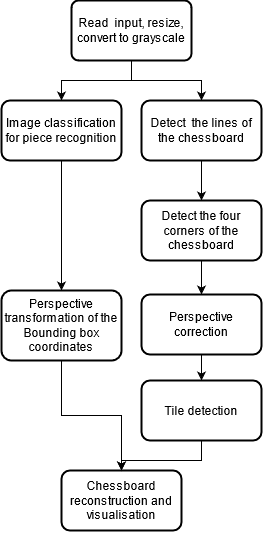
\includegraphics[height=12cm, width=3cm]{Figures/IP-Project-Pipeline-final-left.png}\label{fig:first}}
  \hfill
  \subfloat[Detailed view of the operations which are needed for detecting the chessboard tiles and for performing perspective correction.]{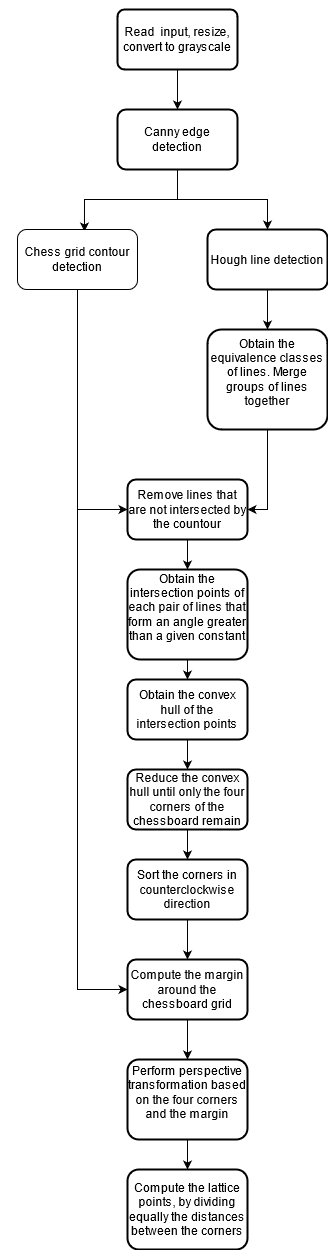
\includegraphics[height=12cm,width=5cm]{Figures/IP-Project-Pipeline-final-right.png}\label{fig:second}}
  \caption{Operation Pipeline}
\end{figure}
%How did you tackle the problem? Here you describe your method in detail and tell us what exactly you have implemented. If your method is in some parts different from the original paper you can explain that here. Include an overview figure that shows your planned processing pipeline.

This paper accompanies a console application which provides a menu for choosing between various operations. The end goal is to take a 3D image of the chessboard and its pieces, and output the corresponding 2D chessboard image. 

In figure \ref{fig:first} is presented the overall operation pipeline. The main steps are to detect the tiles of the chessboard, detect and identify the pieces at each tile, reconstruct the original board and visualise the final result as an image 2D chessboard with pieces.


In this approach a single camera was considered. Moreover the camera does not need to be placed perpendicularly to the board. The intent was to be able to recognise an image taken by a smartphone camera in a given perspective. Camera calibration is an optional step which can be done once, and the resulting camera matrix can be reused in future calculations. There are two possibilities:

\begin{enumerate}
    \item Do the camera calibration with a set of pictures of empty chessboards in different angles. Then this matrix can be used for correcting the image before detecting the lattice points.
    \item Obtain the lattice points of the chessboard for a set of images, do the calibration, then start again the lattice point detection with the now corrected image.
\end{enumerate}

In this program both variants are implemented. In case someone takes its own photographs, pictures with empty chessboards can be taken easily and the result procedure will be simpler. However, in case of images being taken from a dataset which does not contain empty chessboards, then only the second variant can be used.

% This goal is divided into the following subgoals:

% \begin{enumerate}

% \item Detect the corners of the image

% \item Obtain the intrinsic and extrinsic parameters of the camera

% \item Remove the distortions caused by the camera lenses

% \item Obtain a vertical projection of the board

% \item Obtain the tiles of the board

% \item Split the image around each piece

% \item Classify each piece

% \item Visualize the detected chessboard and its pieces in a 2D image.

% \end{enumerate}

We used the pinhole camera model for representing the relationship between world coordinates and image coordinates through the perspective transformation.

\subsection{Corner detection for empty chessboards}
The first topic addressed was the corner detection problem. This represents the main approach in computer vision to draw out features of an object. We applied this mechanism for detecting the corners of an empty chessboard for a given input image. For this step we used the \emph{cv::findChessboardCorners} which takes as parameters the input picture, the size of the image, various operation flags and a vector of 2 dimensional coordinates structure (\emph{Point2f}) in which the function stores the position of all detected corners. In order to have a visual representation of how our approach actually works, we called a predefined function \emph{cv::drawChessboardCorners}. This modifies the source by having the corners colored and connected if the chessboard was successfully detected.

\subsection{Camera calibration}
The lenses of the camera distort the image, thus the last must be pre-processed. The objective of this task is to find the most accurate mapping between the camera image and the perspective camera model. There are two types of lens distortions: \emph{radial}, denoted by \emph{k} and \emph{tangential}, denoted by \emph{p} \cite{2020opencv}.  

Radial distortion implies that some or all the straight lines in the chessboard image appear to be curved. On the other hand, tangential distortion occurs because the image-taking lens is not perfectly parallel aligned to the imaging plane. Therefore, some areas in the image may come across as being nearer than expected \cite{2020opencv}.  

For obtaining the coefficients of the radial distortion we used the following formula:

\begin{center}
\begin{math} 
x_{distorted} = x(1 + k_1r^2 + k_2r^4+ k_3r^6) 
\end{math} 

\begin{math}
y_{distorted} = y(1 + k_1r^2 + k_2r^4+ k_3r^6)
\end{math} 
\end{center}

For the tangential factors we used the following formula: 
\begin{center}
\begin{math} 
 x_{distorted} = x + [2p_1xy + p_2(r^2 + 2x^2)]
\end{math} 

\begin{math}
y_{distorted} = y + [p_1(r^2 + 2y^2) + 2p_2xy]
\end{math}
\end{center}
Some other useful information is connected to the camera parameters: the focal length ($f_x$ - units of horizontal pixels, $f_y$ - units of vertical pixels) and the optical centers ($c_x, c_y$). These represent the intrinsic camera parameters, used to eliminate distortion. The rotation (\begin{math} 
r = 
\begin{bmatrix}
R_x & R_y & R_z
\end{bmatrix}^T\end{math}) and translation (\begin{math} 
t = 
\begin{bmatrix}
T_x & T_y & T_z
\end{bmatrix}^T\end{math}) vectors are the two extrinsic parameters used translate 3D points into the camera coordinate system \cite{slidesNedevschi}. 
\begin{center}
\begin{math} 
Camera\ Matrix = 
 \begin{bmatrix}
f_x & 0 & c_x\\
0 & f_y & c_y\\
0 & 0 & 1
\end{bmatrix}
\end{math} 
\end{center}
The projection equations is: 
\begin{center}
\begin{math} 
\begin{bmatrix}
x\\
y\\
w
\end{bmatrix}
=
\begin{bmatrix}
f_x & 0 & c_x\\
0 & f_y & c_y\\
0 & 0 & 1
\end{bmatrix}
\begin{bmatrix}
X\\
Y\\
Z
\end{bmatrix}
\end{math} 
\end{center}

This implementation loads a set of images, detects their corners and matches them to the 3D chessboard corners. This way we obtain the correspondence between them, which is represented by the above mentioned parameters.

\subsection{Line detection}

If we consider images which have pieces on them, the problem of detecting lattice points becomes much harder because of shadows and hidden corners. Therefore we decided to firstly detect the lines of the chessboard, then find out the intersection points of the horizontal and vertical lines. This way the lattice points are detected even if they are hidden by a piece.

The first step is to detect the lines of chessboard. To do this, the Canny edge detection algorithm is used for obtaining the image with the edges. Before calling the algorithm, a Gaussian blur is applied on the image to smoothen it.

Then the the probabilistic Hough line transform algorithm is used for detecting a list of lines. However for a single line in real life, multiple segments could be detected by this algorithm. Therefore these lines need further processing. First the very small segments are removed. Then the remaining lines are partitioned into equivalency classes based on the relative angles. In the end a reduced list of lines are obtained which appears to be almost ideal.

\subsection{Line cancellation based on the contour of the chessboard grid}

The previously obtained lines are reasonably good. However the image does not contain only the chessboard grid. It can contain other objects whose edges may be detected as lines. For our particular dataset, there is a margin around the chessboard grid which contains markings about the tile coordinates. This way most probably an edge is detected which is outside the grid.

To solve this problem our approach was to obtain the contour of the chessboard grid, then intersect each line with it. Finally keep only those lines which are indeed intersecting with the contour. 

To obtain the contour of the grid, first all contours are found, then the one with the maximum area is kept. This would not be a good solution for any dataset. However for the particular images that was used in this project, the lighting helped to hide some edges of the chessboard margin, thus the largest contour became approximately the chessboard grid.

The next step is to cancel those lines which are not intersecting with the contour. To do this, the contour and the lines are drawn on separate images. Then, for the contour image and for each line images individually, the binary and operator was applied to compute those pixels which are present both in the contour and in the line. If the resulting pixel is all black, there is no intersection and the line can be discarded.

\subsection{Finding the four corners of the chessboard}

The next step is to intersect each horizontal line with each vertical line. To do this, before intersection the angle is verified between the two lines to be greater than a fixed value.

Because line detection may detect more lines than it should, the intersections may provide also some additional points that are not real lattice points. However this is not a problem yet. The goal is now to find the four corners of the chessboard.

First these intersection points are filtered to not have another point in their fixed radius. Then for the remaining points, their convex hull is computed. This convex polygon certainly contains the four corners of the chessboard, given if all four edges of the grid was found by the line detection algorithm.

Then the size of the convex hull is reduced to four elements, by removing those elements whose distance to the line, formed by its immediate neighbors, is smaller then the length of that line. This is repeated in a loop until only the four corners of the chessboard remain.


\subsection{Sort the corners in counterclockwise order and rotate the image}

To obtain  known order of the corners, they are sorted in counterclockwise order. This is achieved by sorting them based on the slope of the line from the corner to the center of mass of the polygon defined by the corner points. After this operation, the corners are in counterclockwise  order, the bottom-right one being on the beginning of the list. 

The image needs to be rotated to a specific orientation, according to the chess rules. The H1 tile was chosen to be placed in the bottom-right corner. To do the rotation, one should rotate the list of corners before doing the perspective correction. Each unit of displacement will result in a turn of 90\textdegree. Therefore the list is rotated once which will correctly position the board.

\subsection{Obtain an optimal margin around the reprojected image}

By doing directly the perspective transformation, the four corners of the board will become the four corners of the image. This way if a piece overlaps the grid, it will be clipped. 

To entail completely all the pieces in the transformed image, a margin is created around the grid, which will also contain the perspective corrected pixels.

To obtain the right dimensions of the margin, the contour points are verified to fit inside the reprojected image. First a perspective correction of the contour point occurs with 0 margin in all directions, based on the corners. Then the bounding rectangle of the contour is verified: if any point of this rectangle is outside the image, the difference is added to the margin of the corresponding direction.

Thus if we redo the perspective correction with the newly computed margin, it will contain completely all the pieces.


\subsection{Perspective transformation and lattice point computation}

The image and the corner points are transformed to achieve perspective correction, by using the \emph{cv::warpPerspective} and \emph{cv:perspectiveTransform} respectively.

If the resulting image is set to be a square, all the lines will become approximately parallel to the image edges, thus the horizontal lines will become approximately perpendicular to the vertical edges. Moreover the size of each tile will be approximately the same.

This important result helps to correctly obtain the corners of the image. The width and height of the image is divided by 8 (the number of tiles in a row/column). This value will be the distance between two consecutive lattice points. Thus with a nested loop all the lattice point positions can be calculated. Moreover the errors in the line or intersection point detection algorithms will not effect the result, given that the four corners are obtained correctly.

Therefore the chessboard is detected, and the four corners of each tile are known.

\subsection{Piece detection}
We used machine learning for detecting the chessboard pieces and we decided that the best approach is to work with \emph{Faster R-CNN} (Region Based Convolutional Neural Networks). As a base for this project iteration we used a web notebook which was modified in order to meet our project's requirements \cite{collab}. The model was trained on the input data set using the TensorFlow Object Detection API. The Faster R-CNN is a two-stage detector which firstly identifies regions of interest and, secondly, feeds these detected regions to a convolutional neural network. Further, the resulting features are passed to \emph{SVM} (Support-Vector Machine) for data classification and regression analysis. Subsequently, the model is exported in a protobuf format, and loaded into the program. For using the model, the Tensorflow C++ API was formerly compiled and linked with the application.

The model receives as input the source image and it returns:

\begin{itemize}
    \item The number of detected objects
    \item The class (piece type) for each detected object
    \item The score for each detected object
    \item Two 2D points per object, defining its bounding box.
\end{itemize}

The detected objects are filtered to keep only those which have a score above a certain threshold.

\subsection{Locating pieces in the final chessboard}

The points of the bounding boxes of each object are transformed through perspective correction, based on the corners. Based on the observation that all the images are taken from the same angle, it was deduced that only the maximum X and Y values of this bounding box must be considered in the computation of the final location. Equation \ref{eqn:piece-location} gives the formula for computing the chessboard location. $x_{top-left}$ is the cx coordinate of the top left corner. $dx$ is the distance between lattice points in the horizontal axis, i.e. the width of a tile. The same formula can be used for computing the y values, by replacing all occurences of x with y, and all width with height.

\newcommand{\round}[1]{\ensuremath{\lfloor#1\rceil}}

\begin{equation}
dx = \frac{width}{8}
\end{equation}

\begin{equation}
\label{eqn:piece-location}
x_{chessboard} = \round{\frac{x_{max} - x_{top-left}}{dx}} - 1
\end{equation}


\subsection{Digital Chessboard Visualization}
After the model is loaded into the program, the detected pieces are added, together with their attributes (class and position), to a storing data structure. Our final representation was developed according to the world-wide recognized standard, therefore, we used the chessboard and piece images previously downloaded from web \cite{chess_piece_board}. Our implementation iterates over every tile of our 512x512 board and in case a piece is found on a certain position, the corresponding digital tile is occupied by the detected chess piece. Because the images are in an \emph{.png} format, for this iteration we took into account only the non-transparent pixels of our matrix representation. 

\section{Evaluation and Results}
%How well does your approach work? Here you show results and explain the experiments you did. Ideally you should have done some evaluation or ablation study that you would present here.
%Run the algorithm on a set of images. Include 1-2 visual results. Also, evaluate the algorithm quantitatively (define or search for performance metrics that show how well your algorithm performs). 

\subsection{Corner detection for empty chessboards}

On figure \ref{fig:corner-detection} one can observe the result of calling the corner detection algorithm on an image from the image set. The chessboard contains 8x5 tiles, which means that it contains 9x6 corners. All the corners of this chessboard were successfully detected, and each vertical line was colored with a different color.

\begin{figure}[bt]
    \centering
    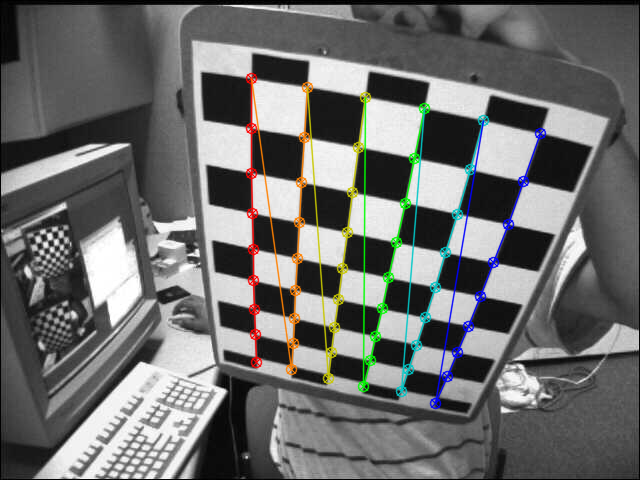
\includegraphics[width=5cm]{Figures/corner-detection.png}
    \caption{The effect of the corner detection. The corners of the chessboard of size 8x5 was detected successfully.}
    \label{fig:corner-detection}
\end{figure}


\subsection{Camera calibration}

One can observe that the edges of the checkerboard are curved in figure \ref{fig:corner-detection}. This radial distortion effect is given by the lenses of the camera which took the photograph. After applying camera calibration the camera matrix and the distortion coefficients are obtained. These matrices are used for undistorting the image. 

The \emph{cv::calibrateCamera} function returns the root mean squared (RMS) error of re-projection \cite{2020opencv}. If this value is closer to 0, the values of the found parameters are more accurate. For the example image of figure \ref{fig:corner-detection} the obtained RMS error is 0.392583.

Figure \ref{fig:camera-calibration} shows the first approach for undistorting an image using the \emph{undistort} function of OpenCV. One can observe that the edges of the chessboard became straight. Another observation is that the image is cropped to have the same size as the input image.

Figure \ref{fig:camera-calibration2} shows the second approach for undistortion, by computings the undistortion and rectification transformation map and remapping the source image. One can observe that the edges of the chessboard are indeed straight, however now the image is not cropped, instead it appears like if someone tried to fold it in half horizontally.

\begin{figure}[bt] 
    \centering
    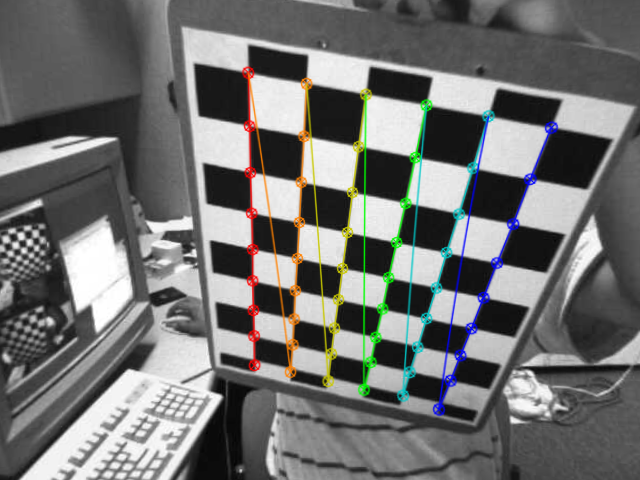
\includegraphics[width=5cm]{Figures/camera-calibration.png}
    \caption{Camera calibration reduces the distortion effect given by the camera lenses. One can observe that all edges of the chessboard became straight. The image is cropped.}
    \label{fig:camera-calibration}
\end{figure}

\begin{figure}[bt] 
    \centering
    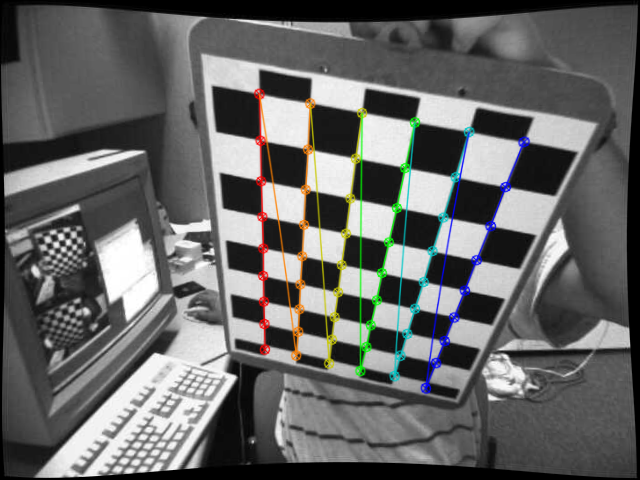
\includegraphics[width=5cm]{Figures/camera-calibration2.png}
    \caption{All the edges of the chessboard became straight. The image appears like it is folded in half horizontally a small amount.}
    \label{fig:camera-calibration2}
\end{figure}


\subsection{Line detection}
\label{sec:line_detection}

Figure \ref{fig:img-gray} shows the input image after it is resized and converted to grayscale.

Figure \ref{fig:img-canny} shows the result of the Canny edge detection. One can observe that the largest contour appears to be indeed the grid of tiles, and not the physical board itself with the margin. This happened because of the lighting of the input image.

Figure \ref{fig:img-hough} shows the result of the Hough line transform algorithm and the detected lines. One can observe that it is not perfect. Because of the white pieces in the leftmost column ate close to the left edge, the algorithm detected multiple lines in that region. In total it detected 38 lines.

Figure \ref{fig:img-reduced} shows the reduced number of lines after the equivalence partitioning algorithm. It is visible that that there are much less lines, the green colored regions is much thinner in the left part of  the board. In total it detected 22 lines;

\begin{figure}[bt] 
    \centering
    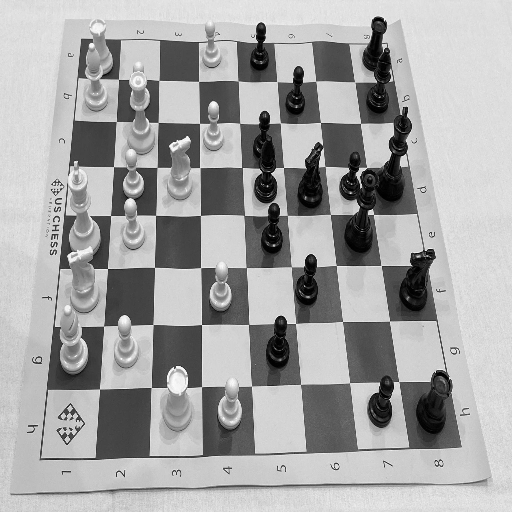
\includegraphics[width=5cm]{Figures/image-gray.png}
    \caption{Input image converted to grayscale}
    \label{fig:img-gray}
\end{figure}



\begin{figure}[bt] 
    \centering
    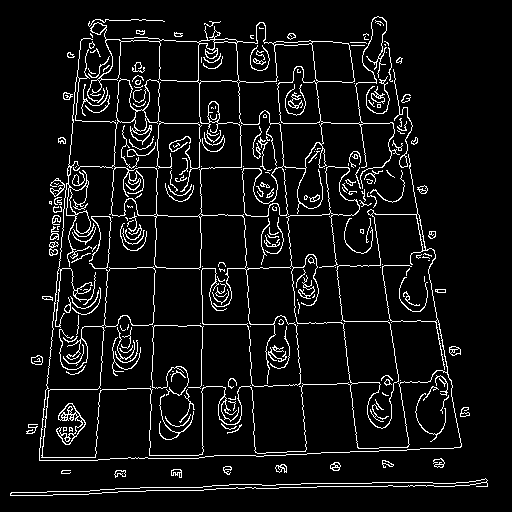
\includegraphics[width=5cm]{Figures/Canny edge detection.png}
    \caption{Result of Canny edge detection}
    \label{fig:img-canny}
\end{figure}

\begin{figure}[bt] 
    \centering
    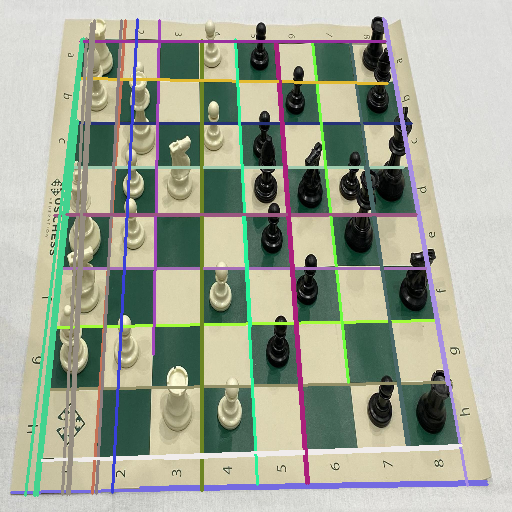
\includegraphics[width=5cm]{Figures/Detected Lines.png}
    \caption{Detected lines by the Hough  line  transform  algorithm}
    \label{fig:img-hough}
\end{figure}

\begin{figure}[bt] 
    \centering
    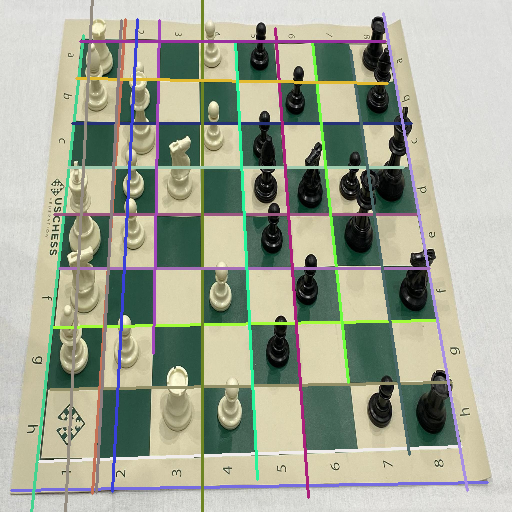
\includegraphics[width=5cm]{Figures/Reduced Lines.png}
    \caption{The reduced number of lines after using the equivalence partitioning algorithm}
    \label{fig:img-reduced}
\end{figure}


\subsection{Line cancellation based on the contour of the chessboard grid}

Figure \ref{fig:img-contour} shows the detected maximum area contour. As mentioned in section \ref{sec:line_detection}, this contour will be approximately the grid of tiles, the edges of the physical board don't appear entirely in the image of detected edges.

Figure \ref{fig:img-filtered} shows the lines after filtering by intersection. It detected 21 lines. The only line which is removed was the bottom edge of the physical board, because it was entirely outside the contour.

After the line detection steps 21 lines were obtained which are more than the optimal number of 18. However this error is resolved in the future steps.


\begin{figure}[bt] 
    \centering
    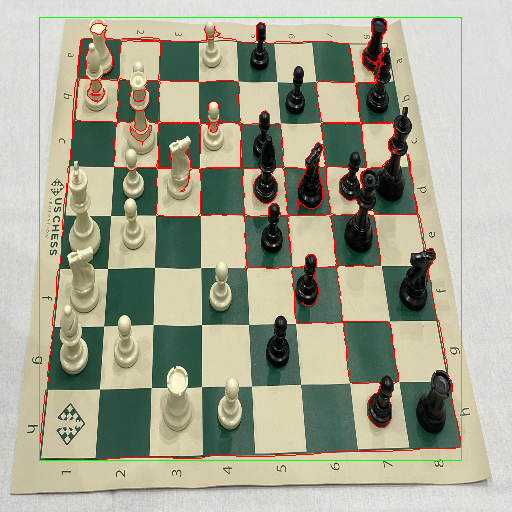
\includegraphics[width=5cm]{Figures/imgWithContours.png}
    \caption{The detected contour}
    \label{fig:img-contour}
\end{figure}

\begin{figure}[bt] 
    \centering
    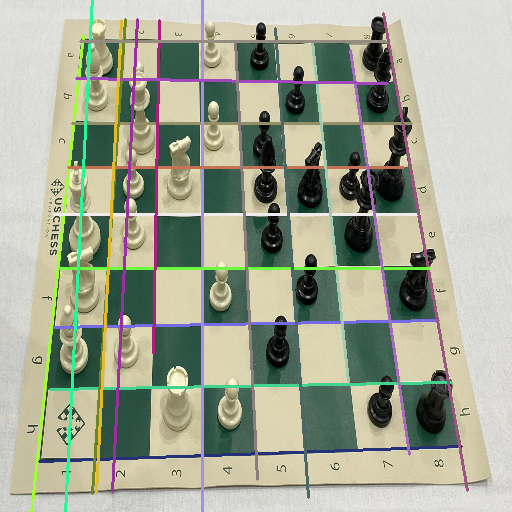
\includegraphics[width=5cm]{Figures/Reduced Lines filtered.png}
    \caption{The filtered lines after checking the intersection with the contour}
    \label{fig:img-filtered}
\end{figure}

\subsection{Finding the four corners of the chessboard}

The horizontal and vertical lines which were detected above are now intersected. Each intersection point is verified to be inside the image, and each pair of lines are verified to have an angle at least 40 degrees. 216 points are obtained. After discarding the points that are in a nearby neighborhood of other points (figure \ref{fig:img-intersection}), 86 points remained. The optimal number is 81. The difference of 5 is obtained because of the 3 lines which were not supposed to be detected. In most of the examples the number of lines were detected correctly in the previous steps, thus in this step the correct number of points were detected.

Again this error will be resolved in the future steps. The current goal is to find the four points of the board which is one of these points.

Figure \ref{fig:img-conex-hull} shows the points of the convex hull. One can observe that indeed the four corners of the board are part of this polygon.

Figure \ref{fig:img-board-corners} shows the result after reducing the size of the convex hull to 4. Thus obtaining the four corners of the chessboard grid.


\begin{figure}[bt] 
    \centering
    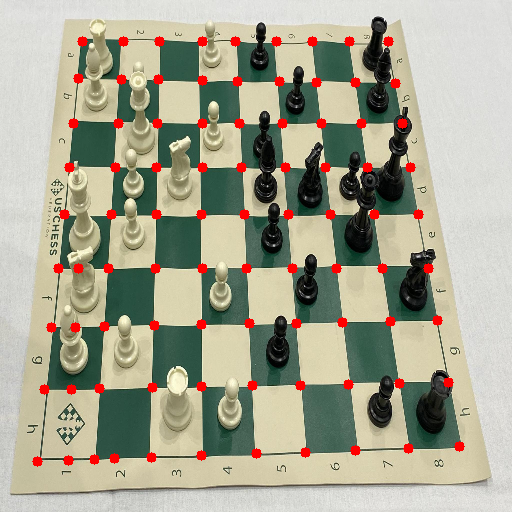
\includegraphics[width=5cm]{Figures/Intersection points.png}
    \caption{The intersection points of horizontal and vertical lines}
    \label{fig:img-intersection}
\end{figure}

\begin{figure}[bt] 
    \centering
    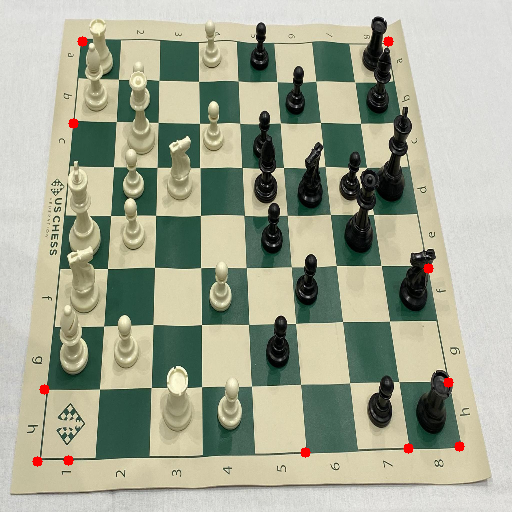
\includegraphics[width=5cm]{Figures/Convex hull of intersection points.png}
    \caption{The convex hull of intersection points}
    \label{fig:img-conex-hull}
\end{figure}

\begin{figure}[bt] 
    \centering
    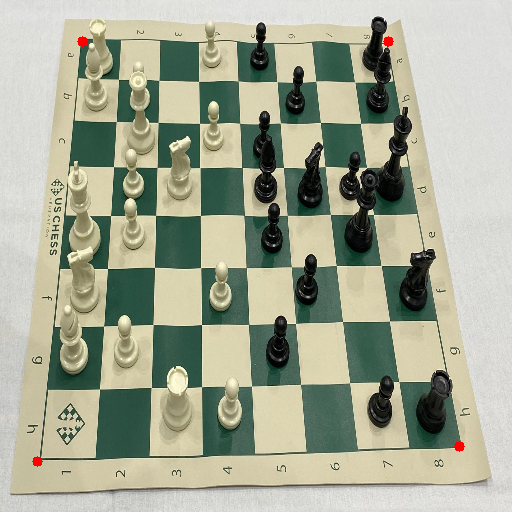
\includegraphics[width=5cm]{Figures/Intersection corners.png}
    \caption{The reduced convex hull results in the four corners of the chessboard grid}
    \label{fig:img-board-corners}
\end{figure}


\subsection{Sort the corners in counterclockwise order and rotate the image}

The program prints to the console the coordinates of the corners (listing \ref{lst:corners}). One can observe that they are indeed in counterclockwise order. After doing the perspective transformation (figure \ref{fig:img-reprojected}) the image will be correctly oriented, because of the rotation of the corners.

\begin{lstlisting}[label={lst:corners},caption={Corner coordinates of the chessboard}]
Corners: [387.931, 41] [82.3471, 41] [36.6344, 461.084] [459.262, 446.062]
\end{lstlisting}


\subsection{Perspective transformation and lattice point computation}

Figure \ref{fig:img-reprojected} shows the image after perspective transformation is applied on it and on its corner points. One can observe that the resulting chessboard is approximately similar to a regular 8x8 grid with equally large cells.

Based on these observations the new points are computed by dividing the horizontal and vertical distances by 8, which will be the approximate sizes of the tiles. On figure \ref{fig:img-reprojected-all} one can observe the result of these calculations, and that it can be considered as a reasonably good result.

One can also observe on figure \ref{fig:img-reprojected-margin} that all the pieces are visible completely. This is achieved by setting the margin to the optimal value.

\begin{figure}[bt] 
    \centering
    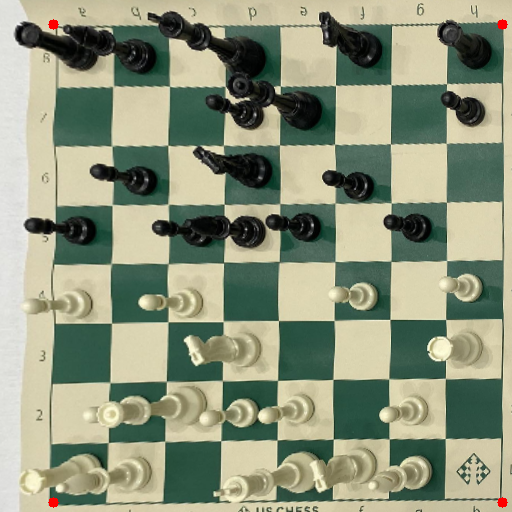
\includegraphics[width=5cm]{Figures/Reprojected image with four corners.png}
    \caption{Projection transformation of the image based on the four corners}
    \label{fig:img-reprojected}
\end{figure}

\begin{figure}[bt]
    \centering
    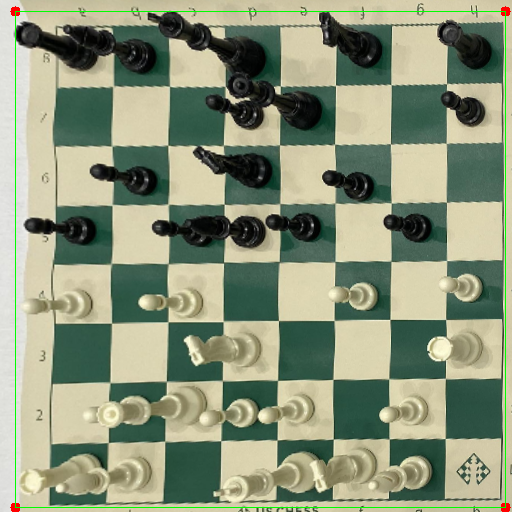
\includegraphics[width=5cm]{Figures/Reprojected image with contour bounding box.png}
    \caption{The bounding box of the contour after perspective correction. One can observe that all figures are visible completely.}
    \label{fig:img-reprojected-margin}
\end{figure}


\begin{figure}[bt] 
    \centering
    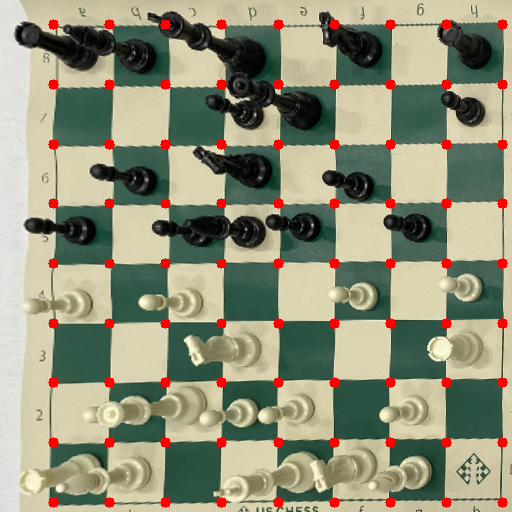
\includegraphics[width=5cm]{Figures/Reprojected image with all lattice points.png}
    \caption{Newly calculated lattice points}
    \label{fig:img-reprojected-all}
\end{figure}


\begin{figure}[!tbp]
  \centering
  \subfloat[Source]{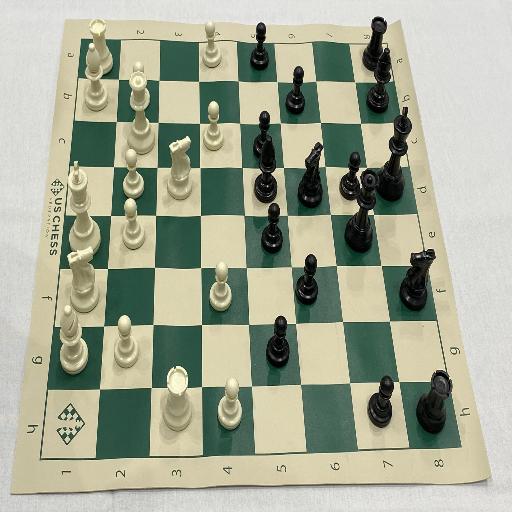
\includegraphics[height=4cm]{Figures/source image.png}\label{fig:a}}
  \hfill
  \subfloat[Predicted pieces]{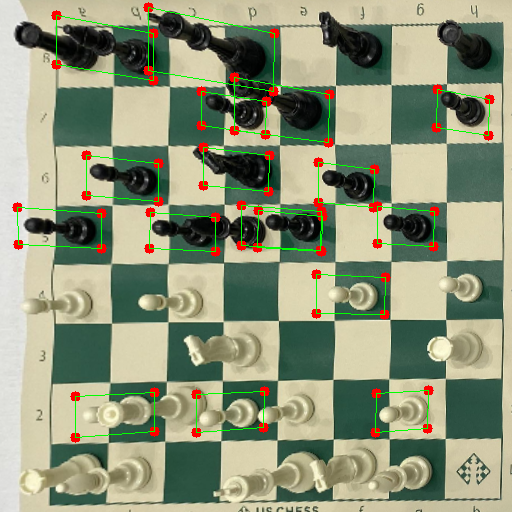
\includegraphics[height=4cm]{Figures/Predicted piece bounding boxes.png}\label{fig:b}}\hfill
  \subfloat[Digital chessboard]{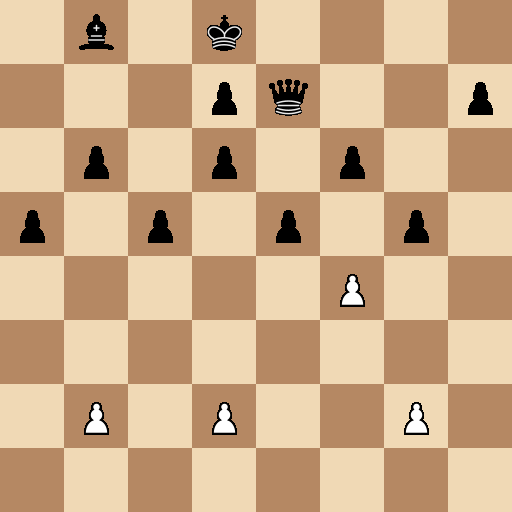
\includegraphics[height=4cm]{Figures/Chessboard.png}\label{fig:c}}
  \caption{Final result visualization}
\end{figure}

\subsection{Piece detection and visualization}

Figure \ref{fig:a} shows the input image, an actual photo of the real chessboard, in \ref{fig:b} one can see the predicted pieces with their bounding boxes while figure \ref{fig:c} shows the final result, the digital representation of the given chessboard.

The model did not predicted perfectly. The causes can be the limited number of training epochs, shadows, piece overlapping and other factors. However it predicted correctly a noticeable number of pieces, thus a relatively good result is obtained.








% An example of a floating figure using the graphicx package.
% Note that \label must occur AFTER (or within) \caption.
% For figures, \caption should occur after the \includegraphics.
% Note that IEEEtran v1.7 and later has special internal code that
% is designed to preserve the operation of \label within \caption
% even when the captionsoff option is in effect. However, because
% of issues like this, it may be the safest practice to put all your
% \label just after \caption rather than within \caption{}.
%
% Reminder: the "draftcls" or "draftclsnofoot", not "draft", class
% option should be used if it is desired that the figures are to be
% displayed while in draft mode.
%
%\begin{figure}[!t]
%\centering
%\includegraphics[width=2.5in]{myfigure}
% where an .eps filename suffix will be assumed under latex, 
% and a .pdf suffix will be assumed for pdflatex; or what has been declared
% via \DeclareGraphicsExtensions.
%\caption{Simulation results for the network.}
%\label{fig_sim}
%\end{figure}

% Note that the IEEE typically puts floats only at the top, even when this
% results in a large percentage of a column being occupied by floats.


% An example of a double column floating figure using two subfigures.
% (The subfig.sty package must be loaded for this to work.)
% The subfigure \label commands are set within each subfloat command,
% and the \label for the overall figure must come after \caption.
% \hfil is used as a separator to get equal spacing.
% Watch out that the combined width of all the subfigures on a 
% line do not exceed the text width or a line break will occur.
%
%\begin{figure*}[!t]
%\centering
%\subfloat[Case I]{\includegraphics[width=2.5in]{box}%
%\label{fig_first_case}}
%\hfil
%\subfloat[Case II]{\includegraphics[width=2.5in]{box}%
%\label{fig_second_case}}
%\caption{Simulation results for the network.}
%\label{fig_sim}
%\end{figure*}
%
% Note that often IEEE papers with subfigures do not employ subfigure
% captions (using the optional argument to \subfloat[]), but instead will
% reference/describe all of them (a), (b), etc., within the main caption.
% Be aware that for subfig.sty to generate the (a), (b), etc., subfigure
% labels, the optional argument to \subfloat must be present. If a
% subcaption is not desired, just leave its contents blank,
% e.g., \subfloat[].


% An example of a floating table. Note that, for IEEE style tables, the
% \caption command should come BEFORE the table and, given that table
% captions serve much like titles, are usually capitalized except for words
% such as a, an, and, as, at, but, by, for, in, nor, of, on, or, the, to
% and up, which are usually not capitalized unless they are the first or
% last word of the caption. Table text will default to \footnotesize as
% the IEEE normally uses this smaller font for tables.
% The \label must come after \caption as always.
%
%\begin{table}[!t]
%% increase table row spacing, adjust to taste
%\renewcommand{\arraystretch}{1.3}
% if using array.sty, it might be a good idea to tweak the value of
% \extrarowheight as needed to properly center the text within the cells
%\caption{An Example of a Table}
%\label{table_example}
%\centering
%% Some packages, such as MDW tools, offer better commands for making tables
%% than the plain LaTeX2e tabular which is used here.
%\begin{tabular}{|c||c|}
%\hline
%One & Two\\
%\hline
%Three & Four\\
%\hline
%\end{tabular}
%\end{table}


% Note that the IEEE does not put floats in the very first column
% - or typically anywhere on the first page for that matter. Also,
% in-text middle ("here") positioning is typically not used, but it
% is allowed and encouraged for Computer Society conferences (but
% not Computer Society journals). Most IEEE journals/conferences use
% top floats exclusively. 
% Note that, LaTeX2e, unlike IEEE journals/conferences, places
% footnotes above bottom floats. This can be corrected via the
% \fnbelowfloat command of the stfloats package.




\section{Conclusion}
% Conclude your work. Restate what problem you have tried to solve, what was original in your work and how well did you manage to achieve the results. You can also suggest future improvements.

The scope of this paper and the accompanying program was to present a method for obtaining a digital representation of a 3D chessboard and its pieces.

The goal was reached partly. The model needs to be further improved to provide better predictions.

Another limitation of our approach is that assumptions were made about the input data. The algorithm is specific to the features of the images:

\begin{itemize}
    \item Camera position. This also implies the elongation direction of the pieces in the image.
    \item Lighting: the maximum contour contains only the chess grid because the lighting makes the borders of the chessboard edges undetectable for the Canny edge detection. 
\end{itemize}

A great achievement from our perspective is that through this project we have broaden our horizons beyond the \emph{Image Processing} domain, due to machine learning integration.
We are looking forward to improving our approach so that a more general solution and a better prediction is obtained.



% trigger a \newpage just before the given reference
% number - used to balance the columns on the last page
% adjust value as needed - may need to be readjusted if
% the document is modified later
%\IEEEtriggeratref{8}
% The "triggered" command can be changed if desired:
%\IEEEtriggercmd{\enlargethispage{-5in}}

% references section

% can use a bibliography generated by BibTeX as a .bbl file
% BibTeX documentation can be easily obtained at:
% http://mirror.ctan.org/biblio/bibtex/contrib/doc/
% The IEEEtran BibTeX style support page is at:
% http://www.michaelshell.org/tex/ieeetran/bibtex/
%\bibliographystyle{IEEEtran}
% argument is your BibTeX string definitions and bibliography database(s)
%\bibliography{IEEEabrv,../bib/paper}
%
% <OR> manually copy in the resultant .bbl file
% set second argument of \begin to the number of references
% (used to reserve space for the reference number labels box)

\nocite{*}

{\small
	\bibliographystyle{plain}
	\bibliography{citations}
}


% \begin{thebibliography}{9}

% \bibitem{1} 
% Wikipedia, 
% \texttt{https://en.wikipedia.org/wiki/Camera\_resectioning}
% %\textit{Camera resectioning} - \textit{https://en.wikipedia.org/wiki/Camera_resectioning} 

% \bibitem{2} 
% Maciej A. Czyzewski, Artur Laskowski, Szymon Wasik, 
% \textit{Chessboard and Chess Piece Recognition With the Support of Neural Networks}

% \bibitem{3} 
% HARRIS, C., AND STEPHENS, M.
% \textit{A combined corner and edge detector} in Alvey vision conference (1988), vol. 15

% \end{thebibliography}


% that's all folks
\end{document}


